
\chapter{Configurazione del \textit{Router}}
\label{ch:configurazione-router}

\section{Overview della configurazione \ok}

In questo capitolo andremo a configurare il \textit{Router 4g} e connetterlo alla VPN.

Continuando a seguire un approccio incrementale, ignoriamo per ora gli \textit{host-domotici} e aggiungiamo alla topologia solo il \textit{Router 4G}. Quindi, la configurazione di partenza sarà descritta in fig.~\ref{fig:conf-init-router}.

\newsavebox{\myimagea}
\begin{figure}[H]
    \centering%
    \savebox{\myimagea}{
        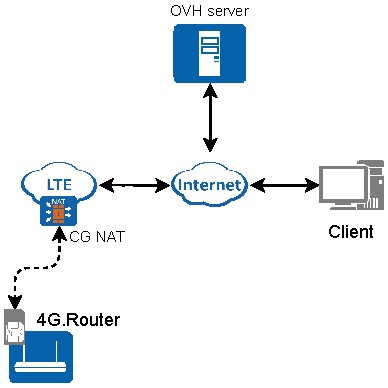
\includegraphics[width=0.45\textwidth]{immagini/diag-router_real}
    }
    \begin{subfigure}{0.4\textwidth}
        \centering
        \usebox{\myimagea}
        \caption{Configurazione iniziale}
        \label{fig:conf-init-router}
    \end{subfigure}
    \hfill%
    \begin{subfigure}{0.5\textwidth}
        \centering
        \raisebox{\dimexpr.5\ht\myimagea-.5\height\relax}{
            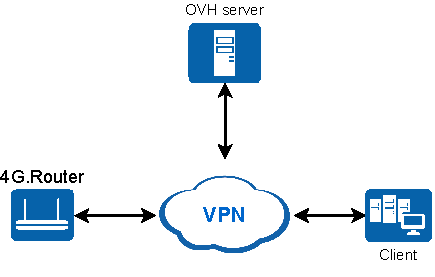
\includegraphics[width=1\linewidth]{immagini/diag-router_goal}
        }
        \caption{Configurazione da raggiungere}
        \label{fig:conf-final-router}
    \end{subfigure}
    \caption{Schemi delle configurazioni iniziali e finali per il capitolo \ref{ch:configurazione-router}.}
\end{figure}

L'obbiettivo di questo capitolo è di configurare il \textit{Router 4G} e il \textit{Server} in modo da poter instaurare un canale di comunicazione tra \textit{Router} e \textit{Client}, raggiungendo una topologia virtuale descritta in fig.~\ref{fig:conf-final-router}.

\section{Prerequisiti per la configurazione del \textit{Router} \ok}

La configurazione del \textit{Router} verrà effettuata sia via shell, sia via interfaccia grafica LuCI, ci si deve assicurare quindi che sia installata (sezione \ref{subsec:luci-web-interface}).

Di default OpenVPN non è presente su OpenWRT, ma lo si può installare usando il package manager. Installiamo inoltre il \href{https://openwrt.org/docs/guide-user/services/vpn/openvpn/client-luci}{plugin di OpenVPN per LuCI}, \code{luci-app-openvpn}.

\begin{bashcode}{Router 4g}{}
$ opkg update
$ opkg install openvpn luci-app-openvpn
\end{bashcode}

\section{Creazione della configurazione OpenVPN per il \textit{Router} \ok}

Per creare il file di configurazione OpenVPN per il \textit{Router} si devono seguire gli step descritti in fig.~\ref{fig:diag-firma_certificato_client}. Supponiamo di usare come \textit{Common Name} \code{router}, quindi dopo aver firmato il certificato e ottenuto il file \code{router.crt} dal \textit{Server CA} possiamo procedere con la creazione della configurazione OpenVPN usando l'apposito script:

\begin{bashcode}{Server}{}
$ ./make_config.sh router
\end{bashcode}

Dopodiché si deve copiare il file \code{router.ovpn} dal \textit{Server} al \textit{Router}, supponiamo di averlo copiato nella cartella \code{/configs} del \textit{Router}. 


\section{Connessione del \textit{Router} alla VPN \ok}

Possiamo quindi spostarci nel \textit{Router} e tentare di connetterlo alla VPN:

\begin{bashcode}{Router 4g}{}
$ openvpn --config /configs/router.ovpn
2022-04-29 17:26:37 OpenVPN 2.5.6 x86_64-openwrt-linux-gnu [SSL (mbed TLS)] [LZ4] [EPOLL] [MH/PKTINFO] [AEAD]
[...]
2022-04-29 17:26:37 VERIFY EKU OK
2022-04-29 17:26:37 VERIFY OK: depth=0, CN=server
2022-04-29 17:26:37 Control Channel: TLSv1.2, cipher TLS-ECDHE-RSA-WITH-AES-256-GCM-SHA384, 2048 bit key
2022-04-29 17:26:37 [server] Peer Connection Initiated with [AF_INET]10.0.4.2:1194
2022-04-29 17:26:37 net_addr_ptp_v4_add: 10.8.0.10 peer 10.8.0.9 dev tun0
2022-04-29 17:26:37 Initialization Sequence Completed
\end{bashcode}

Se il file di configurazione è stato creato correttamente si vedrà il messaggio \\\code{Initialization Sequence Completed}.

Comparirà inoltre l'interfaccia \code{tun0} a cui è assegnato l'indirizzo IP \code{10.8.0.3}.

\section{Auto start del \textit{Client VPN} nel \textit{Router} \ok}

Per abilitare l'avvio automatico del \textit{Client VPN} all'accensione del router si deve, per prima cosa, modificare il file \code{/etc/config/openvpn} in modo che faccia riferimento alla configurazione corretta:

\begin{bashcode}{Router 4g}{}
$ vim /etc/config/openvpn
20  option config /configs/router.ovpn
\end{bashcode}

Ora possiamo abilitarla usando luci:

\begin{figure}[H]
    \centering
    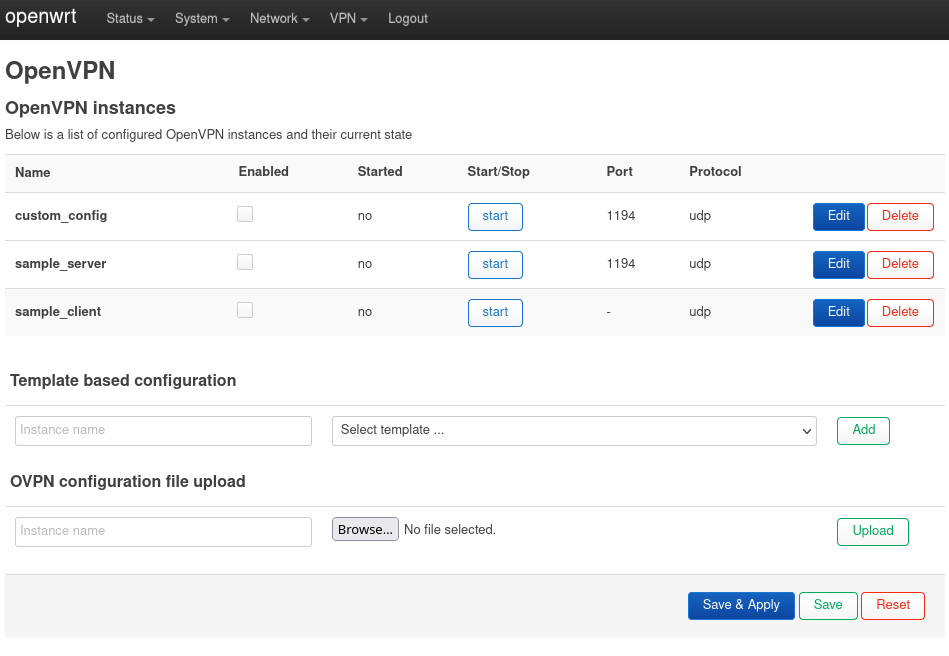
\includegraphics[width=1\textwidth]{immagini/LuCI_vpn1}
    \caption{Configurazione della VPN tramite LuCI.}
    \label{fig:luci-vpn}
\end{figure}

Alla riga "custom\_config" Si deve mettere il check su \textit{enabled} e premere start, per poi salvare le modifiche. In questo modo il router si connetterà automaticamente alla VPN anche se venisse riavviato.


\section{Abilitazione del Client-to-Client nel server OpenVPN \ok}
\label{sec:client-to-client}

In questo momento i client della VPN, \code{client1} e \code{router}, possono comunicare tra loro. Ma lo fanno passando per la network stack del \textit{Server}, possiamo verificarlo con le utility \href{https://en.wikipedia.org/wiki/Ping_(networking_utility)}{\textit{ping}} e \href{https://en.wikipedia.org/wiki/Tcpdump}{\textit{tcpdump}}. 

Eseguiamo ad esempio un test in cui:

\begin{itemize}[nosep, itemsep=1ex]
    \item \code{router} effettua il \textit{ping} verso \code{client1} 
    \item \code{server} è in ascolto sull'interfaccia \code{tun0} usando \code{tcpdump}
\end{itemize}

\begin{bashcode}{Router 4g}{}
$ ping -c1 10.8.0.2                                 # client1
PING 10.8.0.2 (10.8.0.2): 56 data bytes
64 bytes from 10.8.0.2: seq=0 ttl=63 time=0.519 ms
\end{bashcode}

Il \code{ping} ha successo, quindi è possibile una comunicazione bidirezionale tra \code{router} e \code{client1}.

Dal server possiamo vedere un'analisi dei pacchetti che passano attraverso l'interfaccia \code{tun0} usando la utility \code{tcpdump}:

\begin{bashcode}{Server}{}
$ sudo tcpdump -i tun0
listening on tun0, link-type RAW (Raw IP), snapshot length 262144 bytes
16:20:50.791063 IP 10.8.0.3 > 10.8.0.2: ICMP echo request, id 1759, seq 0, length 64
16:20:50.791098 IP 10.8.0.3 > 10.8.0.2: ICMP echo request, id 1759, seq 0, length 64
16:20:50.791273 IP 10.8.0.2 > 10.8.0.3: ICMP echo reply, id 1759, seq 0, length 64
16:20:50.791285 IP 10.8.0.2 > 10.8.0.3: ICMP echo reply, id 1759, seq 0, length 64
\end{bashcode}

\begin{comment} nel caso volessi mette -c2
16:20:51.791153 IP 10.8.0.3 > 10.8.0.2: ICMP echo request, id 1759, seq 1, length 64
16:20:51.791174 IP 10.8.0.3 > 10.8.0.2: ICMP echo request, id 1759, seq 1, length 64
16:20:51.791365 IP 10.8.0.2 > 10.8.0.3: ICMP echo reply, id 1759, seq 1, length 64
16:20:51.791374 IP 10.8.0.2 > 10.8.0.3: ICMP echo reply, id 1759, seq 1, length 64
\end{comment}

Si vede però che ogni richiesta viene duplicata, la prima è in entrata sulla network stack del \textit{Server} e la seconda in uscita. Ciò perché il forwarding del pacchetto viene effettuato dal layer IP del \textit{Server}, e dato che \code{tcpdump} è in ascolto sull'interfaccia \code{tun0}, il pacchetto viene letto 2 volte. Si può vedere una rappresentazione del percorso del pacchetto nella network stack del \textit{Server} in fig.~\ref{fig:diag2-client-to-client-off}, si vede come il pacchetto passa 2 volte per l'interfaccia \code{tun0}, punto 2 e 5. 


\begin{figure}[H]
    \centering
    \begin{subfigure}{0.49\linewidth}
        \centering
        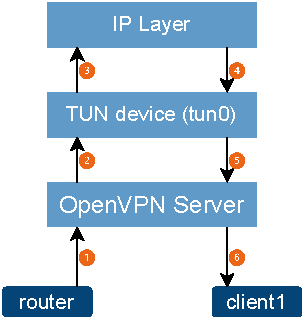
\includegraphics[width=0.8\linewidth]{immagini/diag2-client-to-client-off}
        \caption{Client-to-client off}
        \label{fig:diag2-client-to-client-off}
    \end{subfigure}
    \hfill
    \begin{subfigure}{0.49\linewidth}
        \centering
        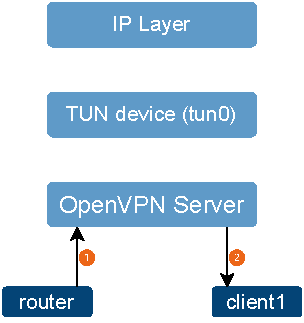
\includegraphics[width=0.8\linewidth]{immagini/diag2-client-to-client-on}
        \caption{Client-to-client on}
        \label{fig:diag2-client-to-client-on}
    \end{subfigure}
    \cprotect\caption{Effetto del \code{client-to-client} sulla network stack del \textit{Server} \cite{client-to-client}.}
\end{figure}


Per evitare questo traffico possiamo abilitare l'opzione \code{client-to-client} nel \textit{Server OpenVPN}. In questo modo il layer OpenVPN effettuerà direttamente il forwarding tra i client della VPN. Graficamente si vede in fig.~\ref{fig:diag2-client-to-client-on} come il pacchetto viene subito inoltrato e non entra affatto nella network stack del server. Ciò comporta, come effetto collaterale, che i pacchetti tra client della VPN non siano soggetti alle regole di firewall imposte nel \textit{Server}.

Andiamo quindi a modificare la configurazione del \textit{Server OpenVPN}:

\begin{bashcode}{Server}{}
$ vim /etc/openvpn/server/server.conf
209  client-to-client
$ sudo systemctl restart openvpn-server@server.service
\end{bashcode}

Possiamo quindi rieseguire gli stessi test fatti sopra:

\begin{bashcode}{Router 4g}{}
$ ping -c1 10.8.0.2                                 # client1
PING 10.8.0.2 (10.8.0.2): 56 data bytes
64 bytes from 10.8.0.2: seq=0 ttl=64 time=0.351 ms
\end{bashcode}

Ma questa volta la network stack del \textit{Server} non vede nessun pacchetto, dato che i pacchetti non passano attraverso l'interfaccia \code{tun0} (fig.~\ref{fig:diag2-client-to-client-on}):

\begin{bashcode}{Server}{}
$ sudo tcpdump -i tun0
listening on tun0, link-type RAW (Raw IP), snapshot length 262144 bytes
\end{bashcode}


\section{Assegnazione IP statico al \textit{Router} \ok}
\label{sec:static-ip-router}

Dato che non possiamo sapere a priori quanti client si connetteranno contemporaneamente alla VPN, e l'assegnazione degli IP da parte del \textit{Server OpenVPN} è dinamico, per conoscere sempre quale IP viene assegnato al \textit{Router} è necessario assegnargliene uno statico attraverso un'opportuna configurazione.

Questo viene fatto usando la \code{client-config-dir}, che consiste in una cartella dove l'amministratore può creare dei file di configurazione specifici per determinati utenti. Ciò è utile in caso alcune configurazioni non debbano essere applicate a tutti gli utenti, ma solo a uno. Il nome del file nella cartella deve essere lo stesso del \textit{Common Name} del certificato del client per cui si sta creando la configurazione.

Nel nostro caso siamo interessati a impostare un IP statico per il \textit{Router}, quindi si deve creare nella cartella \code{ccd} un file chiamato \code{router}. 

L'opzione che permette di impostare un IP statico attraverso la \code{client-config-dir} è \\\code{ifconfig-push} \cite{ifconfig-push}:

\begin{bashcode}{Server}{}
$ sudo mkdir /etc/openvpn/server/ccd         # creo la client-config-dir
$ sudo vim /etc/openvpn/server/ccd/router
ifconfig-push 10.8.0.254 255.255.255.0       # impongo l'ip per questo common name
$ sudo vim /etc/openvpn/server/server.conf   # abilito l'opzione nella config del server
167  client-config-dir ccd
$ sudo systemctl restart openvpn-server@server.service
\end{bashcode}

Così facendo al router gli verrà sempre assegnato l'IP \code{10.8.0.254}, indipendentemente dall'ordine in cui gli host si connettono alla vpn. Ciò ci permette di sapere sempre e a priori qual è l'IP del router.
